%\begin{itemize}
%	\item Based on a graphics pipeline:
%	\item as this is needed for each unit(vertex, primitive, fragment and pixel) independently, this is the of one core.
%\end{itemize}

As graphics processing units or GPUs have matured since the late 1980s their main purpose of displaying the user interface and rendering images has been basically unchanged. Though how they are rendering images has changed the basic structure of GPUs of 2005~\cite{kilgariff2005geforce} are fundamentally the same as the are seen in modern GPUs from today~\cite{nvidia2018turing}.

%PLACEHOLDER: Change the image to the new one
\begin{figure}[H]
	\centering
	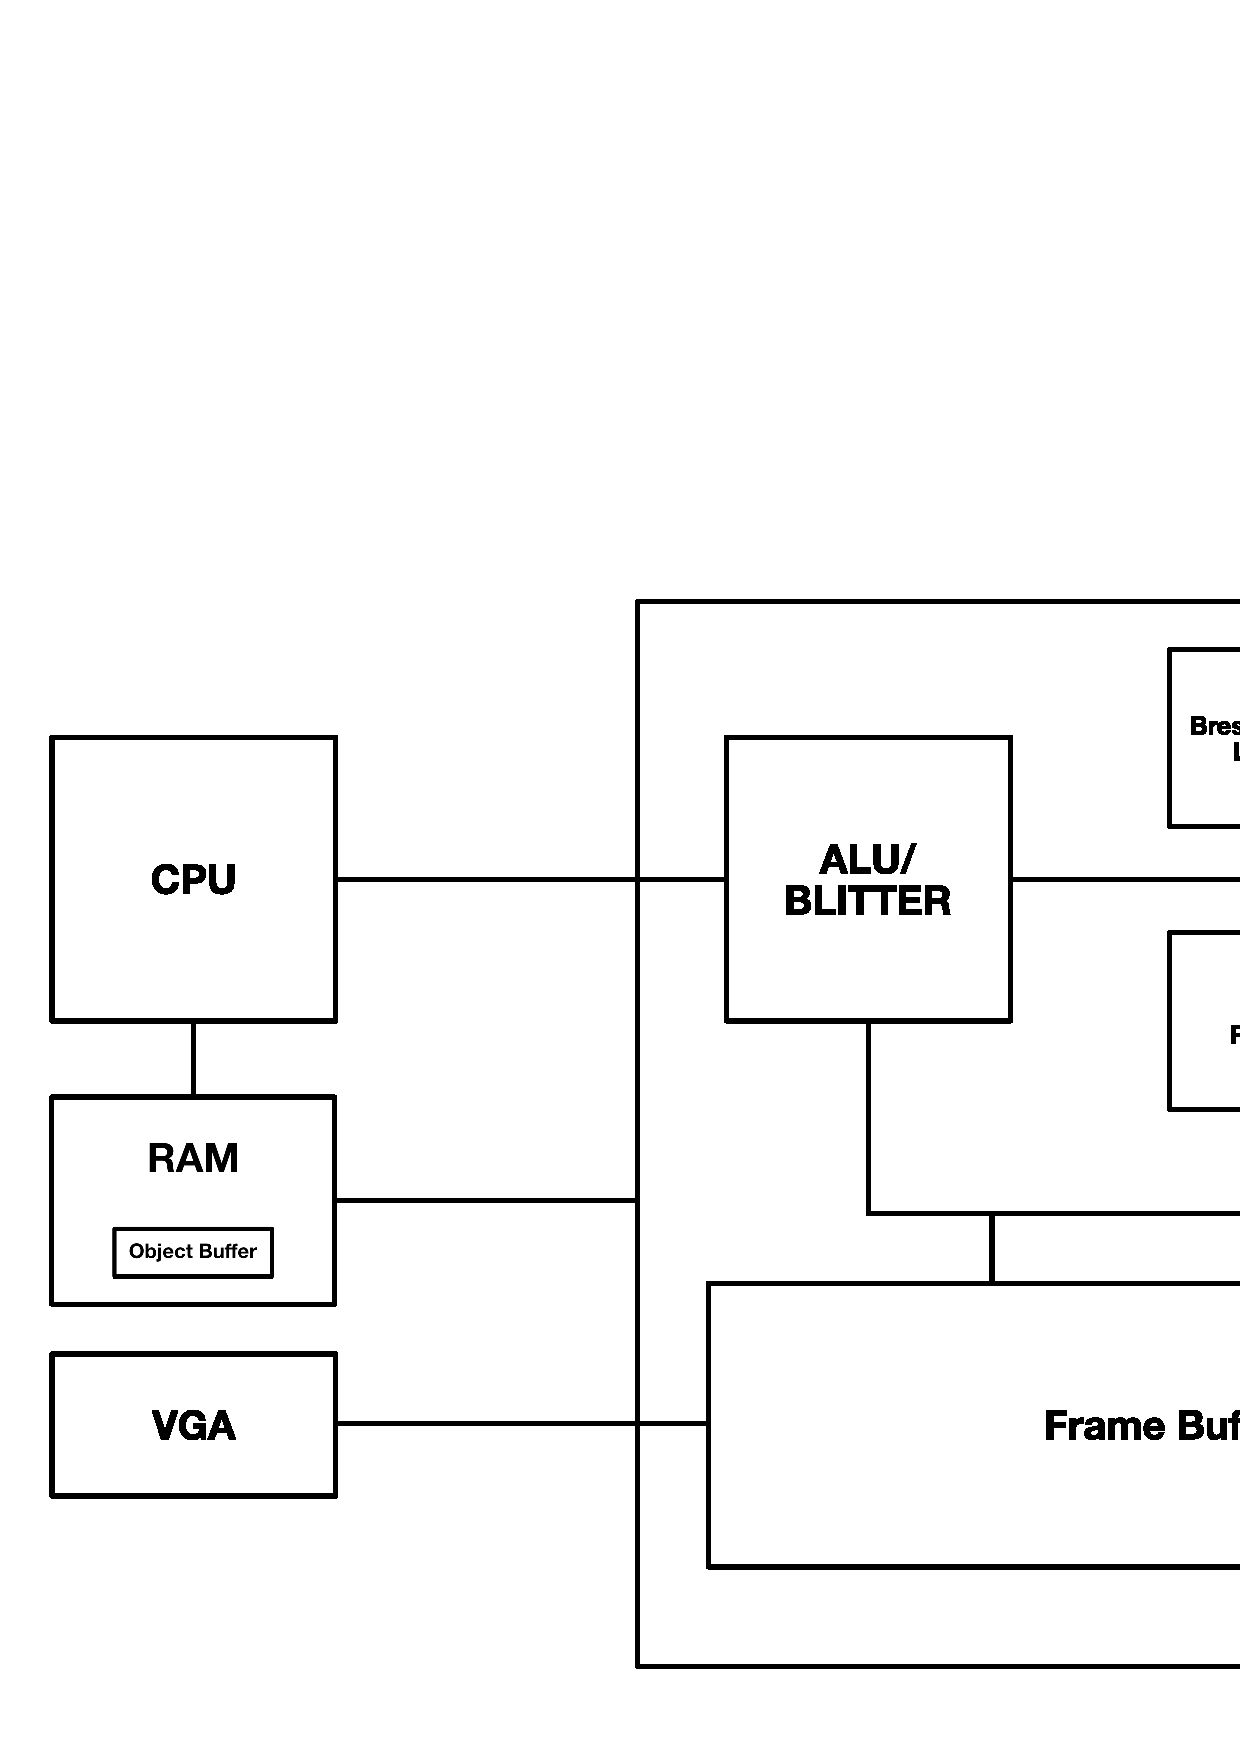
\includegraphics[width=0.5\textwidth]{coredesign}
	\caption{The structure of a GPU pipeline}
	\label{img:gpuPipe}
\end{figure}

The basic structure of how a GPU operates can be seen in \cref{img:gpuPipe}. This pipeline shows the basic functionality of a single core. Each core starts with the processing the vertices. It takes a three dimensional vertex and projects it into screen space, a two dimensional area that gets rendered to the screen. Each vertex is independently projected by a core. In modern computer graphics this process is directed by a vertex shader.

After a vertex is projected into screen space, they are grouped together into logical units that form a triangle. These units are called primitives. They are clipped and culled, where only that is drawn that is visible and facing the screen space, to reduce the processing time needed for the later stages of the pipeline. Those primitives are then rasterized into so called pixel fragments. A pixel fragment is a group of pixels without any color information. To create the color each fragment needs to be shaded to create the visible pixels. Before they are rendered to the screen each fragment is blended into the frame at their pixel location. To determine if a fragment is visible a so called z-buffer is used to determine the drawing order to the frame. This section is handled by a so called fragment shader. 

A modern GPU can consist now of up to 2944 such cores \footnote{As taken from \url{https://www.nvidia.com/en-us/geforce/20-series/} on the sixteenth of September of 2019} that all act in somewhat of the previously described functionality.
